\documentclass[border=4pt]{standalone}
\usepackage{tikz}
\usetikzlibrary{arrows.meta,bending,shapes.geometric}
\begin{document}
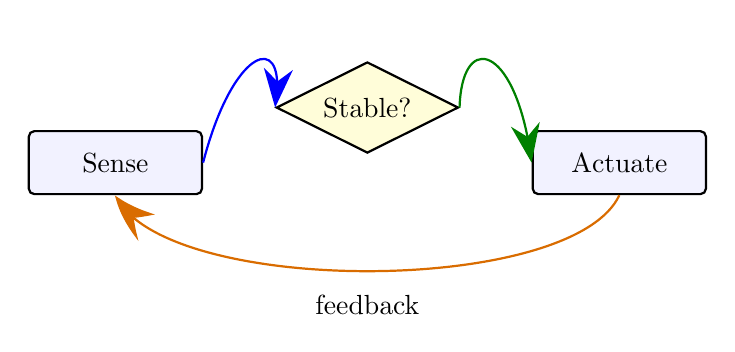
\begin{tikzpicture}[
  process/.style={draw,rounded corners=2pt,minimum width=22mm,minimum height=8mm,fill=blue!5},
  decision/.style={draw,diamond,aspect=2,minimum width=22mm,minimum height=8mm,fill=yellow!15},
  every path/.style={line width=.8pt}
]
  \node[process] (sense) at (0,0) {Sense};
  \node[decision] (check) at (3.2,0.7) {Stable?};
  \node[process] (act) at (6.4,0) {Actuate};

  \draw[blue,-{Stealth[length=14pt,flex]}]
    (sense.east) .. controls (1.5,1.5) and (2.2,1.7) .. (check.west);
  \draw[green!50!black,-{Stealth[length=14pt,flex'=.75]}]
    (check.east) .. controls (4.4,1.7) and (5.1,1.5) .. (act.west);
  \draw[orange!85!black,-{Stealth[length=15pt,bend]}]
    (act.south) .. controls (5.8,-1.7) and (0.6,-1.7) .. (sense.south);
  \node[below] at (3.2,-1.55) {feedback};
\end{tikzpicture}
\end{document}
